\documentclass{standalone}

\usepackage{setspace}
\usepackage{times}
\usepackage{amsmath}
\usepackage{amssymb}
\usepackage{xparse}
\usepackage{ifthen}

\usepackage[dvipsnames]{xcolor}
\usepackage{tikz}
\usetikzlibrary{arrows,calc,patterns,patterns.meta}
\pgfdeclarelayer{background}
\pgfdeclarelayer{foreground}
\pgfsetlayers{background,main,foreground}

\usepackage{pgfplots}
\pgfplotsset{compat=1.15}

\definecolor{plainred}{HTML}{ff0000}
\definecolor{red}{HTML}{972e21}
\definecolor{yellow}{HTML}{ebb83f}
\definecolor{blue}{HTML}{5e7fbf}
\renewcommand{\seriesdefault}{\bfdefault}
\renewcommand{\familydefault}{\sfdefault}

\pgfdeclarepattern{
	name=hatch,
	parameters={\hatchsize,\hatchangle,\hatchlinewidth},
	bottom left={\pgfpoint{-\hatchlinewidth}{-\hatchlinewidth}},
	top right={\pgfpoint{\hatchsize+\hatchlinewidth}{\hatchsize+\hatchlinewidth}},
	tile size={\pgfpoint{\hatchsize}{\hatchsize}},
	tile transformation={\pgftransformrotate{\hatchangle}},
	code={
		\pgfsetlinewidth{\hatchlinewidth}
		\pgfpathmoveto{\pgfpoint{-\hatchlinewidth}{-\hatchlinewidth}}
		\pgfpathlineto{\pgfpoint{\hatchsize+\hatchlinewidth}{\hatchsize+\hatchlinewidth}}
		\pgfusepath{stroke}
	}
}
\tikzset{
	hatch size/.store in=\hatchsize,
	hatch angle/.store in=\hatchangle,
	hatch line width/.store in=\hatchlinewidth,
	hatch size=0.9cm,
	hatch angle=0cm,
	hatch line width=0.2cm,
}

\begin{document}
	\Large%
	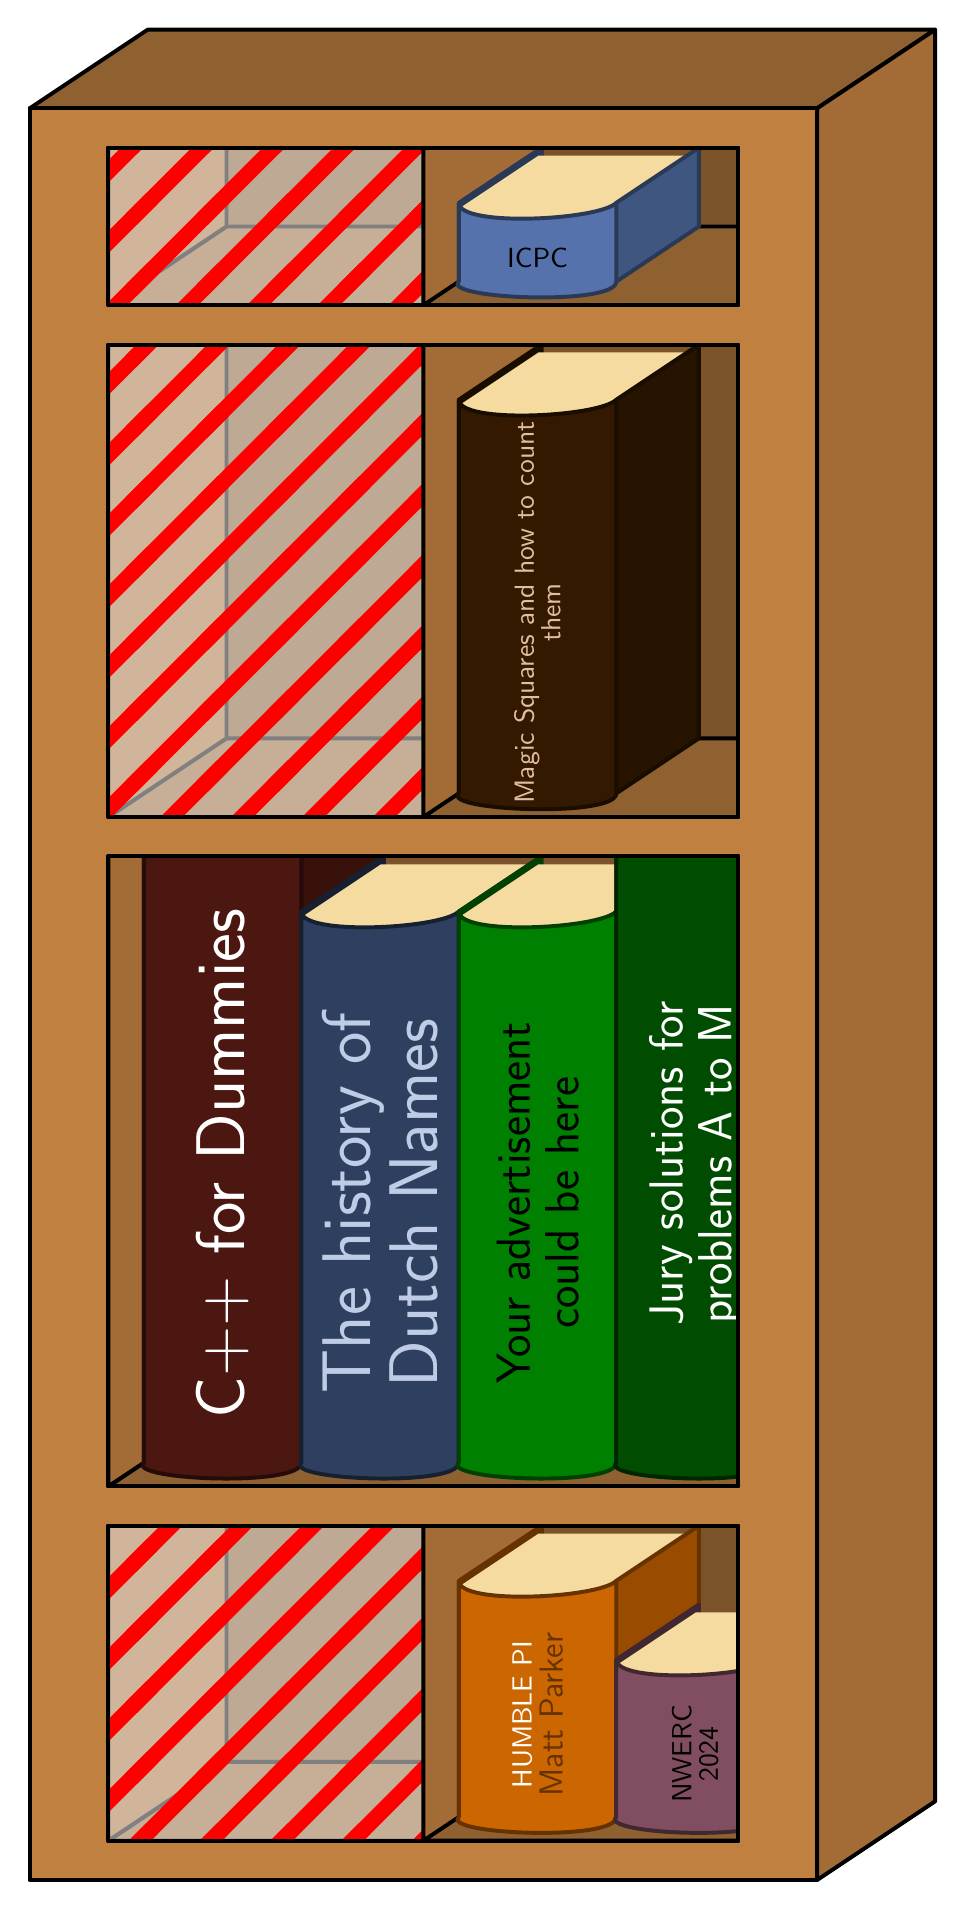
\begin{tikzpicture}[x=2cm,y=1cm,z={(1.5cm,1cm)},line join=round, line cap=round,line width=0.05cm]
		\newcommand{\w}{4}
		\newcommand{\depth}{0.3}
		\newcommand{\rack}[2]{%y,h
			\fill[fill=brown!65!black] (0,#1) rectangle (\w,#1+#2);%back
			\begin{scope}
				\clip (0,#1) rectangle (\w,#1+#2);
				\draw[fill=brown!75!black] (0,#1,0) -- (0,#1,1) -- (\w,#1,1) -- (\w,#1,0) -- cycle;%bottom
				\draw[fill=brown!85!black] (0,#1,0) -- (0,#1,1) -- (0,#1+#2,1) -- (0,#1+#2,0) -- cycle;%left side
			\end{scope}
			\draw (0,#1) rectangle (\w,#1+#2);
		}
		\newcommand{\shelf}{
			\draw[fill=brown!75!black] (\w+0.5,22,0) -- (\w+0.5,22,1) -- (-0.5,22,1) -- (-0.5,22,0) -- cycle;
			\draw[fill=brown!85!black] (\w+0.5,-0.5,0) -- (\w+0.5,-0.5,1) -- (\w+0.5,22,1) -- (\w+0.5,22,0) -- cycle;
			\draw[fill=brown] (-0.5,-0.5) rectangle (\w+0.5,22);
			
			\rack{0.0}{4}
			\rack{4.5}{8}
			\rack{13.0}{6}
			\rack{19.5}{2}
		}
		\newcommand{\book}[4][]{%text,color,x,h			
			\filldraw[#2!50!black] (#3,#4,\depth) -- (#3,#4,1) -- (#3,0,1) -- (#3,0,\depth) -- cycle;%left back side
			\fill[yellow!50] (#3,#4-.0750,\depth) -- (#3,#4-0.5,\depth) -- (#3+1,#4-0.5,\depth) -- (#3+1,#4-0.075,\depth) -- (#3+1,#4-0.075,1-0.025) -- (#3,#4-0.075,1-0.025) -- cycle;%pages top
			\draw[#2!50!black,fill=#2!75!black] (#3+1,0,\depth) -- (#3+1,0,1) -- (#3+1,#4,1) -- (#3+1,#4,\depth) -- cycle;%right side
			%\draw[#2!50!black,fill=#2] (#3,0,\depth) rectangle (#3+1,#4,\depth);%front
			\draw[#2!50!black,fill=#2] (#3,0,\depth) to[in=270,out=270-45,looseness=0.4] (#3+1,0,\depth) -- (#3+1,#4,\depth) to[in=270,out=270-45,looseness=0.4] (#3,#4,\depth) -- cycle;%front
			%deko
			\pgfmathparse{#4<2?0:90}
			\node[rotate=\pgfmathresult,anchor=center,inner sep=0cm,outer sep=0cm] at (#3+0.5,0.5*#4-0.2,\depth) {
				\ifthenelse{#4<2}{\begin{minipage}{2cm}}{\begin{minipage}{#4cm}}
					\setstretch{0.8}\centering
					#1
				\end{minipage}
			};
		}
		\newcommand{\sep}[1]{%x
			\fill[white,opacity=0.5] (0,0) rectangle (#1,100);
			\fill[pattern=hatch, pattern color=plainred] (0,0) rectangle (#1,100);
			\filldraw[black,fill=brown!85!black] (#1,0,0) -- (#1,0,1) -- (#1,100,1) -- (#1,100,0) -- cycle;
		}
		\NewDocumentEnvironment{rackClip}{m m}{
			\begin{scope}[shift={(0,#1)}]
				\clip (0,0) rectangle (\w,#2);
		}{
			\end{scope}
			\draw (0,#1) rectangle (\w,#1+#2);
		}
		
%		\begin{scope}[shift={(0,0)}]
%			\shelf
%			\begin{rackClip}{4.5}{8}
%				\book[\Huge\color{white}C++ for Dummies]{red!50!black}{0}{8}
%				\book[\Huge\color{blue!40}The history of\\Dutch Names]{blue!50!black}{1}{7}
%				\book[\LARGE{}Your advertisement\\could be here]{green!50!black}{2}{7}
%				\book[\LARGE{}\color{white}Jury solutions for\\problems A to M]{green!30!black}{3}{8}
%			\end{rackClip}
%			\begin{rackClip}{13.0}{6}
%				\book[\color{white}HUMBLE PI\\\color{orange!40!black}\large{}Matt Parker]{orange!80!black}{0}{3}
%				\book[NWERC\\2024]{red!60!blue}{1}{2}
%				\book[ICPC]{blue!90!black}{2}{1}
%				\book[\color{brown!50}Magic Squares and how to count them]{orange!20!black}{3}{5}
%			\end{rackClip}
%		\end{scope}
		
		\begin{scope}[shift={(7,0)}]
			\shelf
			\begin{rackClip}{0}{4}
				\sep{2}
				\book[\color{white}HUMBLE PI\\\color{orange!40!black}\large{}Matt Parker]{orange!80!black}{2}{3}
				\book[NWERC\\2024]{red!60!blue}{3}{2}
			\end{rackClip}
			\begin{rackClip}{4.5}{8}
				\book[\Huge\color{white}C++ for Dummies]{red!50!black}{0}{8}
				\book[\Huge\color{blue!40}The history of\\Dutch Names]{blue!50!black}{1}{7}
				\book[\LARGE{}Your advertisement\\could be here]{green!50!black}{2}{7}
				\book[\LARGE{}\color{white}Jury solutions for\\problems A to M]{green!30!black}{3}{8}
			\end{rackClip}
			\begin{rackClip}{13.0}{6}
				\sep{2}
				\book[\color{brown!50}Magic Squares and how to count them]{orange!20!black}{2}{5}
			\end{rackClip}
			\begin{rackClip}{19.5}{2}
				\sep{2}
				\book[ICPC]{blue!90!black}{2}{1}
			\end{rackClip}
		\end{scope}		
	\end{tikzpicture}
\end{document} 
